\documentclass{article} % For LaTeX2e
\usepackage{nips13submit_e,times}
\usepackage{hyperref}
\usepackage{url}
\usepackage{amsmath}
\usepackage{amsfonts}
\usepackage{breakurl}
\usepackage{graphicx}
\usepackage{caption}
\usepackage{subcaption}
\usepackage{float}
\usepackage{fancyvrb}
\usepackage{booktabs}
\usepackage[font=footnotesize,labelfont=bf]{caption}
% \documentstyle[nips13submit_09,times,art10]{article} % For LaTeX 2.09
\bibliographystyle{ieeetr}

\title{Modeling and Simulating Political Violence and Optimizing Aid Distribution in Uganda}


\author{
Peter J.~Bull \\
Institute for Applied Computational Science\\
Harvard University\\
52 Oxford Street \\
Cambridge, MA 02139 \\
\texttt{bull@fas.harvard.edu} \\
\And
Isaac M.~Slavitt \\
Institute for Applied Computational Science\\
Harvard University\\
52 Oxford Street \\
Cambridge, MA 02139 \\
\texttt{slavitt@fas.harvard.edu} \\
}

% The \author macro works with any number of authors. There are two commands
% used to separate the names and addresses of multiple authors: \And and \AND.
%
% Using \And between authors leaves it to \LaTeX{} to determine where to break
% the lines. Using \AND forces a linebreak at that point. So, if \LaTeX{}
% puts 3 of 4 authors names on the first line, and the last on the second
% line, try using \AND instead of \And before the third author name.

\newcommand{\fix}{\marginpar{FIX}}
\newcommand{\new}{\marginpar{NEW}}

\nipsfinalcopy % Uncomment for camera-ready version

\begin{document}


\maketitle

\begin{abstract}
Using MCMC techniques, we model civil conflict in Uganda and optimize the limited relief aid that can be provided in these scenarios. We describe a method to simulate civil conflict events in space and time given historical data about these events. We also optimize the distribution of limited aid resources to refugees from these crises. Modeling aid delivery as a combination of the traveling salesman problem and the knapsack algorithm --- two NP-hard problems --- we find acceptable solutions using stochastic metaheuristics.
\end{abstract}

\section*{The Data}

The data comes from ACLED (Armed Conflict Location and Event Data Project), which is a dataset with locations, dates, fatalities, motivation, actors involved, and other information about civil conflicts in Africa. Their collection of data on Uganda covers 1997-2013, and they have a real-time tracker of events reported in 2014.\cite{ACLED} The need for an understanding of these patterns of conflict is clear, as ACLED notes:

\begin{quote}
This dataset codes the dates and locations of all reported political violence events in over 50 developing countries. Political violence includes events that occur within civil wars or periods of instability. Although civil war occurrence is decreasing across African countries, new forms of political violence are becoming more common.
\end{quote}

\begin{table}[H]
\caption{The ACLED Uganda Dataset}
\centering
\resizebox{\columnwidth}{!}{%
\begin{tabular}{lrlrlrrrr}
\toprule
{} &  GWNO & EVENT\_DATE &  TIME\_PRECISION &                     EVENT\_TYPE &  LATITUDE &  LONGITUDE &  GEO\_PRECIS &  FATALITIES \\
\midrule
0 &   500 & 1997-01-01 &               3 &  Battle-No change of territory &   0.50000 &   32.00000 &           3 &           5 \\
1 &   500 & 1997-01-01 &               3 &  Battle-No change of territory &   2.76667 &   32.30556 &           3 &           4 \\
2 &   500 & 1997-01-07 &               1 &  Battle-No change of territory &   0.13580 &   30.36360 &           1 &           5 \\
3 &   500 & 1997-01-08 &               1 &  Battle-No change of territory &   0.18333 &   30.08333 &           3 &           2 \\
4 &   500 & 1997-01-11 &               1 &     Violence against civilians &   3.12583 &   32.91972 &           1 &           0 \\
\bottomrule
\end{tabular}
}
\end{table}


For Uganda, the dataset contains around 4,500 observations of civil violence. Each observation includes the data, location, an quantified estimate for how precise these measures are, a number of fatalities for the event, and the actors involved. Figure \ref{fig:map-points} shows these conflicts scattered on a political map of Uganda.

\begin{figure}
  \centering
  \begin{subfigure}[b]{0.5\textwidth}
    \centering
    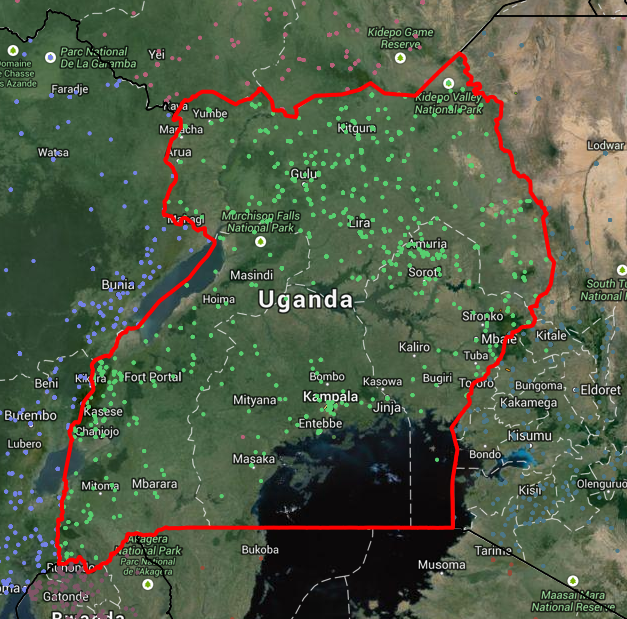
\includegraphics[width=\textwidth]{figures/uganda}
    \caption{Civil conflicts in Uganda 1997-2013.}
    \label{fig:map-points}
  \end{subfigure}~\begin{subfigure}[b]{0.5\textwidth}
    \centering
    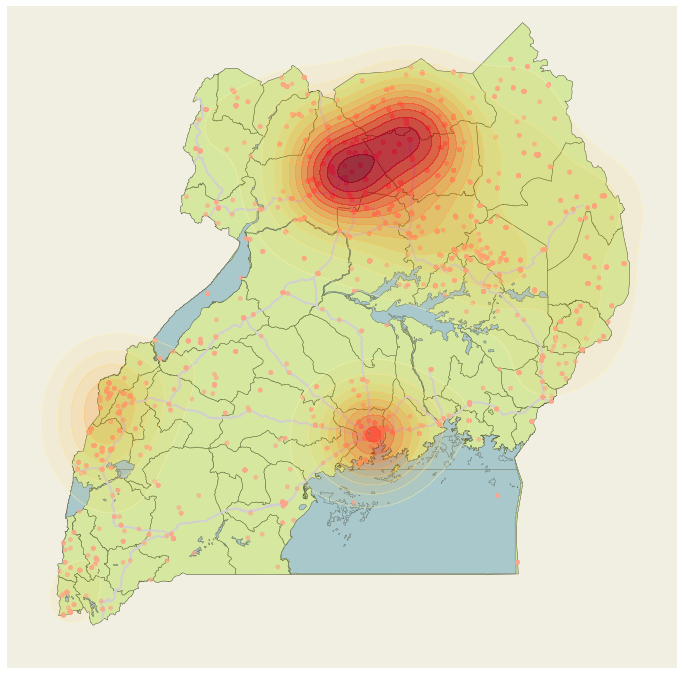
\includegraphics[width=\textwidth]{figures/map-with-smoothed-data}
    \caption{Conflicts with Mat\'{e}rn smoothing.}
    \label{fig:map-smoothed}
  \end{subfigure}
  \caption{Civil conflicts in Uganda.}
  \label{fig:map}
\end{figure}


\section*{Modeling civil conflict}

\subsection*{Events in space}

The events of violence and civil conflict that are available from the ACLED dataset are coded with both a latitude and a longitude. One assumption we make is that these events are distributed due to underlying causes such as population centers, road access, historical land ownership, and other features that make conflicts more or less likely. It is difficult to get the data and create a generative model for these probabilities, so we make the assumption that the distribution of the data is representative of these factors. In effect, we treat the entire country of Uganda as a probability distribution from which geospatial conflict events could be sampled.  We took historical conflict location data from the entire ACLED data set and smoothed it using a Mat\'{e}rn covariance function.  Figure \ref{fig:map-smoothed} shows this smoothing applied to the same conflicts depicted in \ref{fig:map-points}.

We used this smooth as a kernel-density esitmate. This estimate (i.e., the empirical distribution of the conflict data), has a complex functional form which makes it challenging to sample from. However, it is simple for a given coordinate to get the probability of an event. Given this property of our smooth, we can apply monte-carlo sampling techniques to generate samples from this probability distribution. Visualizing the distribution, we see that it is multi-modal with regions of low density between the modes. Because of these properties, we opted to use slice sampling to generate draws from the distribution. Figure \ref{fig:sampled-conflicts} shows the first 1,000 samples from this probability distribution (note, as some point we could write code to throw away samples that occur over water or outside of country boundaries). Figure \ref{fig:histogram} shows the distribution of the samples as a two-dimensional histogram.

\begin{figure}
  \centering
  \begin{subfigure}[b]{0.5\textwidth}
    \centering
    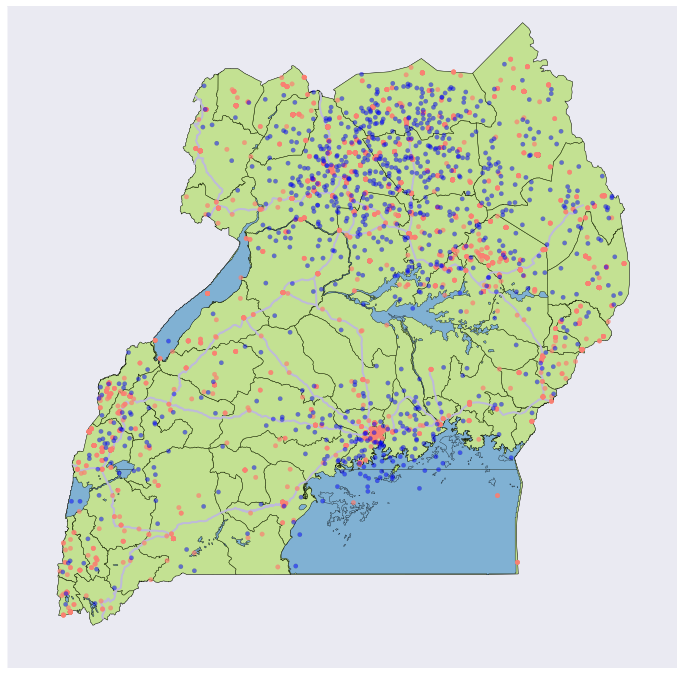
\includegraphics[width=\textwidth]{figures/1000-slice-samples}
    \caption{Blue dots are samples from the empirical distribution.}
    \label{fig:sampled-conflicts}
  \end{subfigure}~\begin{subfigure}[b]{0.5\textwidth}
    \centering
    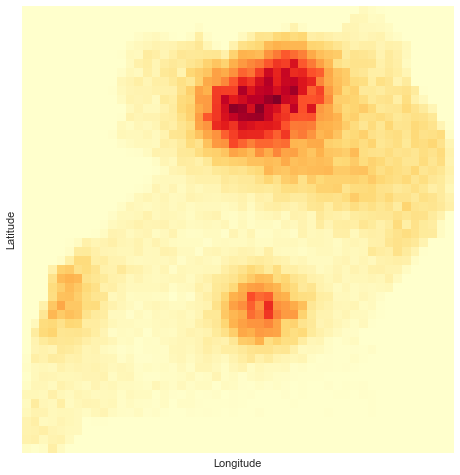
\includegraphics[width=\textwidth]{figures/histogram}
    \caption{2d histogram of slice samples from the empirical distribution.}
    \label{fig:histogram}
  \end{subfigure}
\end{figure}

When slice sampling, there are a number of parameter choices that are imporant. We want to choose our rectangle widths, burn-in, and thinning parameters appropriately. In testing, a thinning value of 10 reduced autocorrelation to less than 0.1 at a time lag of 1. We can see this result in Figure \ref{fig:autocorr}. We used the Gelman-Rubin potential scale reduction factor \cite{Gelman-Rubin} to determine if we were mixing well. Generally, a value less than 1.1 indicates good mixing. In both of our dimensions, the Gelman-Rubin statistic was less than this threshold. We also calculated the Gewecke statistic, which is used to indicate convergence. A value less than 2 indicates convergence and for our draws, this statisic was $\ll$ 1. We can also examine convergence by looking at the trace plots for the samples. As we see in Figure \ref{fig:trace} these appear stationary.

\begin{figure}
  \centering
  \begin{subfigure}[b]{0.5\textwidth}
    \centering
    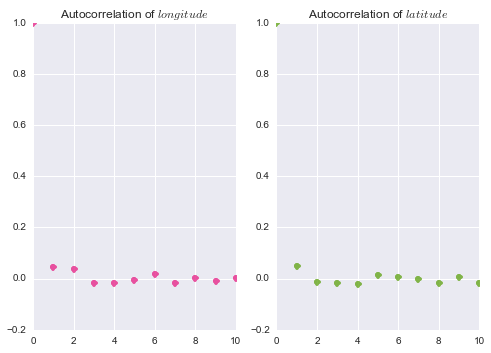
\includegraphics[width=\textwidth]{figures/autocorr-latlong}
    \caption{Autocorrelation for the samples from latitude and longitude}
    \label{fig:autocorr}
  \end{subfigure}~\begin{subfigure}[b]{0.5\textwidth}
    \centering
    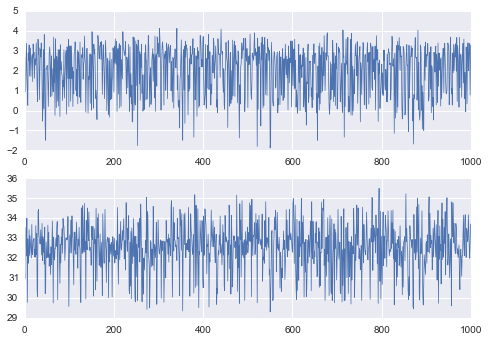
\includegraphics[width=\textwidth]{figures/trace-plots}
    \caption{Trace plots for draws from the latitude and longitude}
    \label{fig:trace}
  \end{subfigure}
\end{figure}

\subsection*{Events in time}
As a modeling assumption, we seperate the dimensions of space and time as being independent. To model events in time across the country, we use an autoregressive Poisson GLM. While standard autoregressive models create a linear relation between a future value and a previous value, the Poisson GLM lets us have a linear relation between previous data and the mean of a Poisson distribution. This will allow us to retain the probabilistic interpretation of the events in time.

In order to model events using a Poisson distribution, we must discretize our time dimension. We opted for month-long increments. The thinking behind this decision is that we want to use sample draws to run our aid optimizations. If a model like this were to be used in planning for future conflicts, having a month-long window for a plan seems like a good balance between precision and logistic concerns.

\emph{TODO:} Finish code and incorporate results.

\subsection*{Putting it together}
We can now use our draws in space and time to generate a simulation of further conflicts in Uganda. These simulated scenarios will be the basis of our adaptive aid-placement and allocation optimization. A model of conflict events in space and time, along with optimized aid-delivery could help organizations such as the Red Cross to order supplies, allocate staff and volunteers, and develop infrastructure.

\section*{Optimizing Resource Placement and Allocation}

In the second part of this project, we use the first section as both inspiration for the aid delivery analogy and also as a source of randomly sampled data points representing geospatially distributed conflicts.

\subsection*{The Traveling Salesman Problem}

One question of particular interest that we can tackle using techniques from the class is how to route emergency aid
to locations where it is needed.  For concreteness, let's postulate a Red Cross medical or food supply caravan that originates
from the organization's in-country headquarters. This caravan wishes to visit all $n$ emergent locations in order to
deliver needed supplies. They wish to do so in the most efficient manner possible.

This is fundamentally an optimization problem, and one that is well known -- it was first described in 1932 by Karl Menger (shortly after his year here at Harvard as a visiting lecturer) and has been studied extensively ever since.\cite{Menger} Here is the traditional convex optimization specification of the problem:\cite{Winston}


\begin{align*}
\min &\sum_{i=0}^n \sum_{j\ne i,j=0}^nc_{ij}x_{ij} &&  \\
\mathrm{s.t.} & \\
	& x_{ij} \in \{0, 1\} && i,j=0, \cdots, n \\
	& \sum_{i=0,i\ne j}^n x_{ij} = 1 && j=0, \cdots, n \\
	& \sum_{j=0,j\ne i}^n x_{ij} = 1 && i=0, \cdots, n \\
	&u_i-u_j +nx_{ij} \le n-1 && 1 \le i \ne j \le n
\end{align*}

As is clear from the specification, this is an integer linear program (ILP) where:

\begin{itemize}
  \item $x_{ij}$ is a binary decision variable indicating whether we go from location $i$ to location $j$.
  \item $c_{ij}$ is the distance between location $i$ and location $j$.
  \item The objective function is the sum of the distances for routes that we decide to take.
  \item The final constraint ensures that all locations are visited once and only once.
\end{itemize}

\subsection*{Answering complex, realistic questions}

\subsubsection*{Packing the aid truck - adding the Knapsack Problem}

We extend the TSP into a multi-objective optimization problem
where \emph{the contents of the aid trucks} also have an optimization component. Therein lies
the knapsack problem: subject to a volume or weight constraint, and given that different locations
might have very different needs such as food, vaccinations, or emergent medical supplies, \emph{which
supplies do we pack on the trucks}?

Here's the unbounded\footnote{Often, this problem is formulated such that you can only bring one of
each item, but that doesn't make sense here. We want to be able to bring as many types of each type
of aid as we think necessary, and we'll assume that as many as desired are available to load on the
trucks before starting out from HQ.} version of the knapsack problem:

\begin{align*}
\max &\sum_{i=1}^n v_i x_i &&  \\
\mathrm{s.t.} & \\
    & x_i \in \mathbb{Z} \\
    & x_i \geq 0 \\
	& \sum_{i=1}^n w_ix_i \leq W
\end{align*}

In this formulation:

\begin{itemize}
  \item $x_{i}$ is a zero or positive integer decision variable indicating how many units of item $i$
        we load on the truck.
  \item $v_i$ is the utility we get from bringing along item $i$.
  \item $w_i$ is the weight of item $i$.
  \item $W$ is the maximum weight the truck can carry.
\end{itemize}

The problem, of course, is that brute force solution of the TSP is $\mathcal{O}$$(n!)$. Traditional, deterministic
algorithm approaches such as branch-and-bound or branch-and-cut are still impractical for larger numbers of nodes.
In many cases, exhaustive search for global optimality is not even particularly helpful as long as the solution
found is good enough. We will use simulated annealing (SA) to get acceptable solutions to the TSP (c.f. the class lectures
and homework problem).

\begin{figure}
  \centering
  \begin{subfigure}[b]{0.5\textwidth}
    \centering
    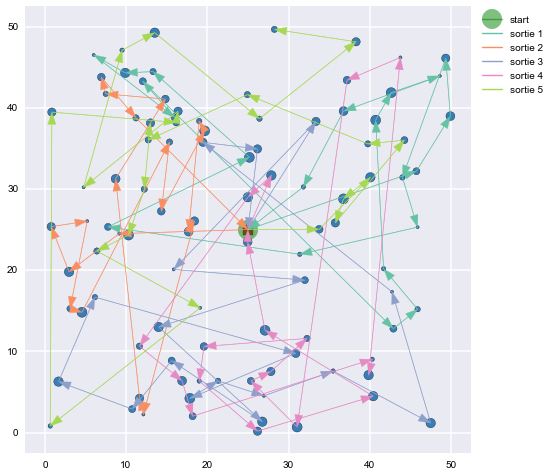
\includegraphics[width=\textwidth]{figures/sorties-5000}
    \caption{After 5,000 iterations.}
  \end{subfigure}~\begin{subfigure}[b]{0.5\textwidth}
    \centering
    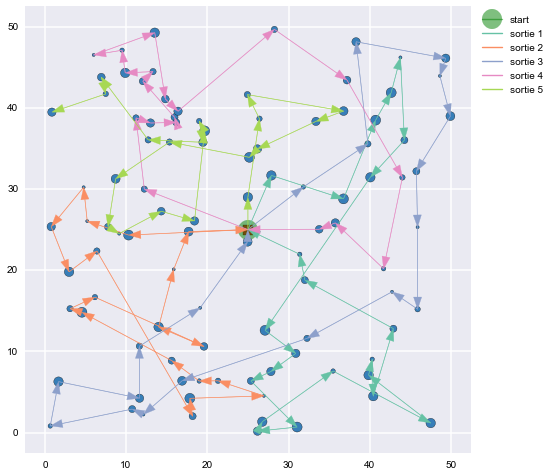
\includegraphics[width=\textwidth]{figures/sorties-20000}
    \caption{After 20,000 iterations.}
  \end{subfigure}
  \begin{subfigure}[b]{\textwidth}
    \centering
    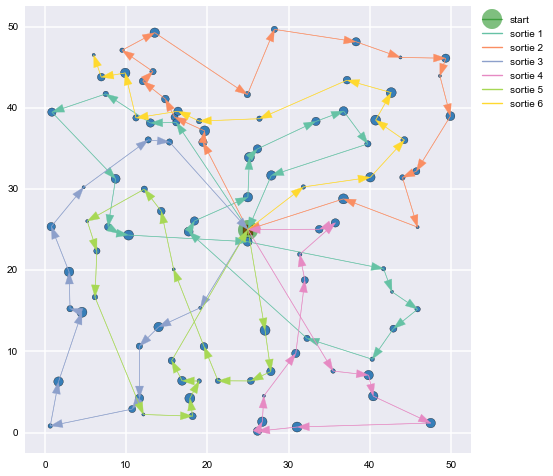
\includegraphics[width=\textwidth]{figures/sorties-100000}
    \caption{After 100,000 iterations.}
  \end{subfigure}
  \caption{Routing for the TSP/Knapsack hybrid.}
  \label{fig:sorties}
\end{figure}

\begin{figure}
	\centering
	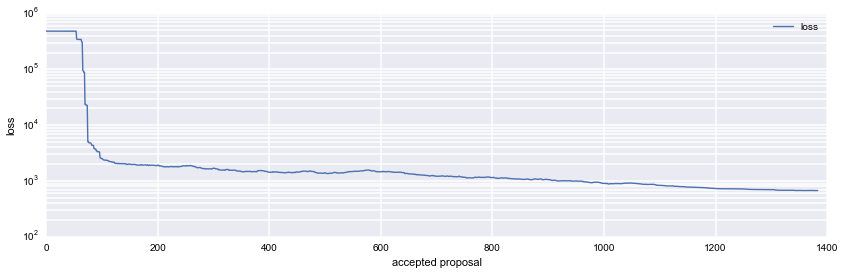
\includegraphics[width=\textwidth]{figures/sorties-loss}
	\caption{Loss function acceptances over 100,000 iterations.}
	\label{fig:sorties-loss}
\end{figure}

\subsubsection*{Finding the optimal site for the resupply location}

\emph{TODO:} At the moment, our code draws random cities. We need to update this code to use the samples from our slice sampling instead.

\emph{TODO:} We are working on the code that incorporates finding the optimal location of HQ.

\subsubsection*{Factoring in travel time and loss from service delays}

Since we have draws in space and time, we want to update our cost function. As refugees build up, injuries go untreated, and citizens become more desperate for supplies, sending the aid truck to a particular location becomes more important. We want to incorporate this idea by including a time-sice-event term in our cost function. As time passes and the site remains unvisited, it becomes more important for the aid truck to visit these locations. 

\emph{TODO:} Incorporate this code and results.

\bibliography{proposal}

\end{document}
